\documentclass[border=3pt,tikz]{standalone}
\usepackage{bm,amsmath}
\usetikzlibrary{patterns,decorations.pathmorphing}
\usetikzlibrary{arrows.meta}
\usetikzlibrary{calc}

\begin{document}

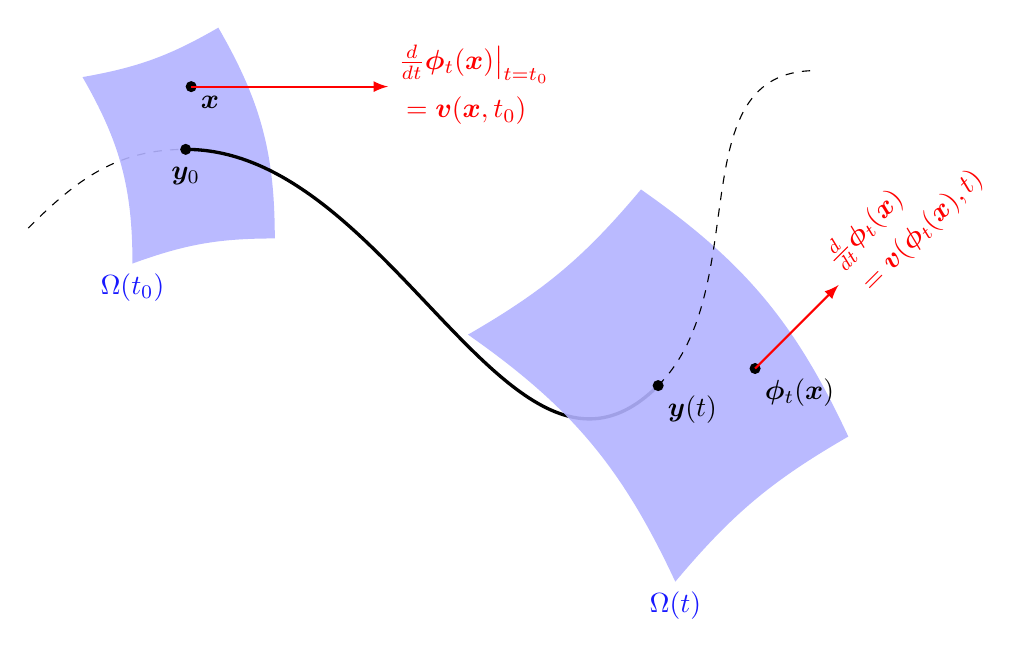
\begin{tikzpicture}
    \def\angXzero{0}
    \def\angXone{45}
    \def\rzero{1.6}
    \def\rone{2.5}
    
    \coordinate (A)  at (-1,0);
    \coordinate (Xzero) at (1,1);
    \coordinate (Xone) at (7,-2);
    \coordinate (B)  at (9,2);

    \draw[dashed] (A) to[out=45, in=180+\angXzero] (Xzero);
    
    \fill[blue!30,opacity=0.9] ($(Xzero)+(75:\rzero)$) to[bend left=10] ($(Xzero)+(145:\rzero)$) to[bend left=15] ($(Xzero)+(65:-\rzero)$) node[blue, below] {$\Omega(t_0)$} to[bend left=10] ($(Xzero)+(135:-\rzero)$) to[bend right=15] cycle;
    
    \draw[very thick] (Xzero) to[out=\angXzero,in=180+\angXone] (Xone);

    \fill[blue!30,opacity=0.9] ($(Xone)+(95:\rone)$) to[bend left=10] ($(Xone)+(165:\rone)$) to[bend left=15] ($(Xone)+(95:-\rone)$) node[below,blue] {$\Omega(t)$} 
    to[bend left=10] ($(Xone)+(165:-\rone)$) to[bend right=15] cycle;

    \draw[dashed] (Xone) to[out=\angXone,in=180] (B);

    \coordinate(X) at ($(Xzero)+(85:0.5*\rzero)$);
    \fill (X) circle (2pt) node[below right] {$\bm{x}$};
    \draw[-latex, red, thick] (X) -- ++(\angXzero:2.5) 
        node[right, sloped, pos=1] {$\begin{aligned}&\tfrac{d}{dt}\bm{\phi}_t(\bm{x})\big|_{t=t_0}\\&=\bm{v}(\bm{x},t_0)\end{aligned}$};
        

    \coordinate (Y) at ($(Xone)+(10:0.5*\rone)$);
    \fill (Y) circle (2pt) node[below right] {$\bm{\phi}_t(\bm{x})$};
    \draw[-latex, red, thick] (Y) -- ++(\angXone:1.5) 
        node[right, sloped, pos=1] {$\begin{aligned}&\tfrac{d}{dt}\bm{\phi}_t(\bm{x})\\&=\bm{v}(\bm{\phi}_t(\bm{x}),t)\end{aligned}$};


    \fill (Xzero) circle (2pt) node[below=3pt] {$\bm{y}_0$};
    \fill (Xone) circle (2pt) node[below right] {$\bm{y}(t)$};
                
\end{tikzpicture}

\end{document}
